\section{Was ist Graphentheorie?}

Die Graphentheorie ist ein Zweig der Mathematik, der mit der Untersuchung von Graphen befasst ist, wobei es sich um Strukturen handelt, die aus Knoten (eng. Nodes, auch Punkte genannt) und Kanten (eng. Edges, auch Bögen oder Linien genannt) bestehen, die die Knoten verbinden.
Graphen sind ein nützliches Werkzeug zum Modellieren und Verstehen der Beziehungen zwischen verschiedenen Objekten oder Entitäten und sie haben zahlreiche Anwendungen in einer Vielzahl von Bereichen,
darunter Informatik, Ingenieurwesen, Biologie und Soziologie \cite[p.~1ff.]{bollobas_modern_1998}.

Auf Abbildung \ref{fig:overview_indices} folgt eine Übersicht, in welcher die Arbeit verschiedenen Feldern der Lehre und Forschung angegliedert wird.
Sie zeigt Schnittstellen zu diversen Bereichen und gibt den Zusammenhang der topologischen Indizes zu anderen Themen wieder.

\begin{figure}[H]
    \centering
    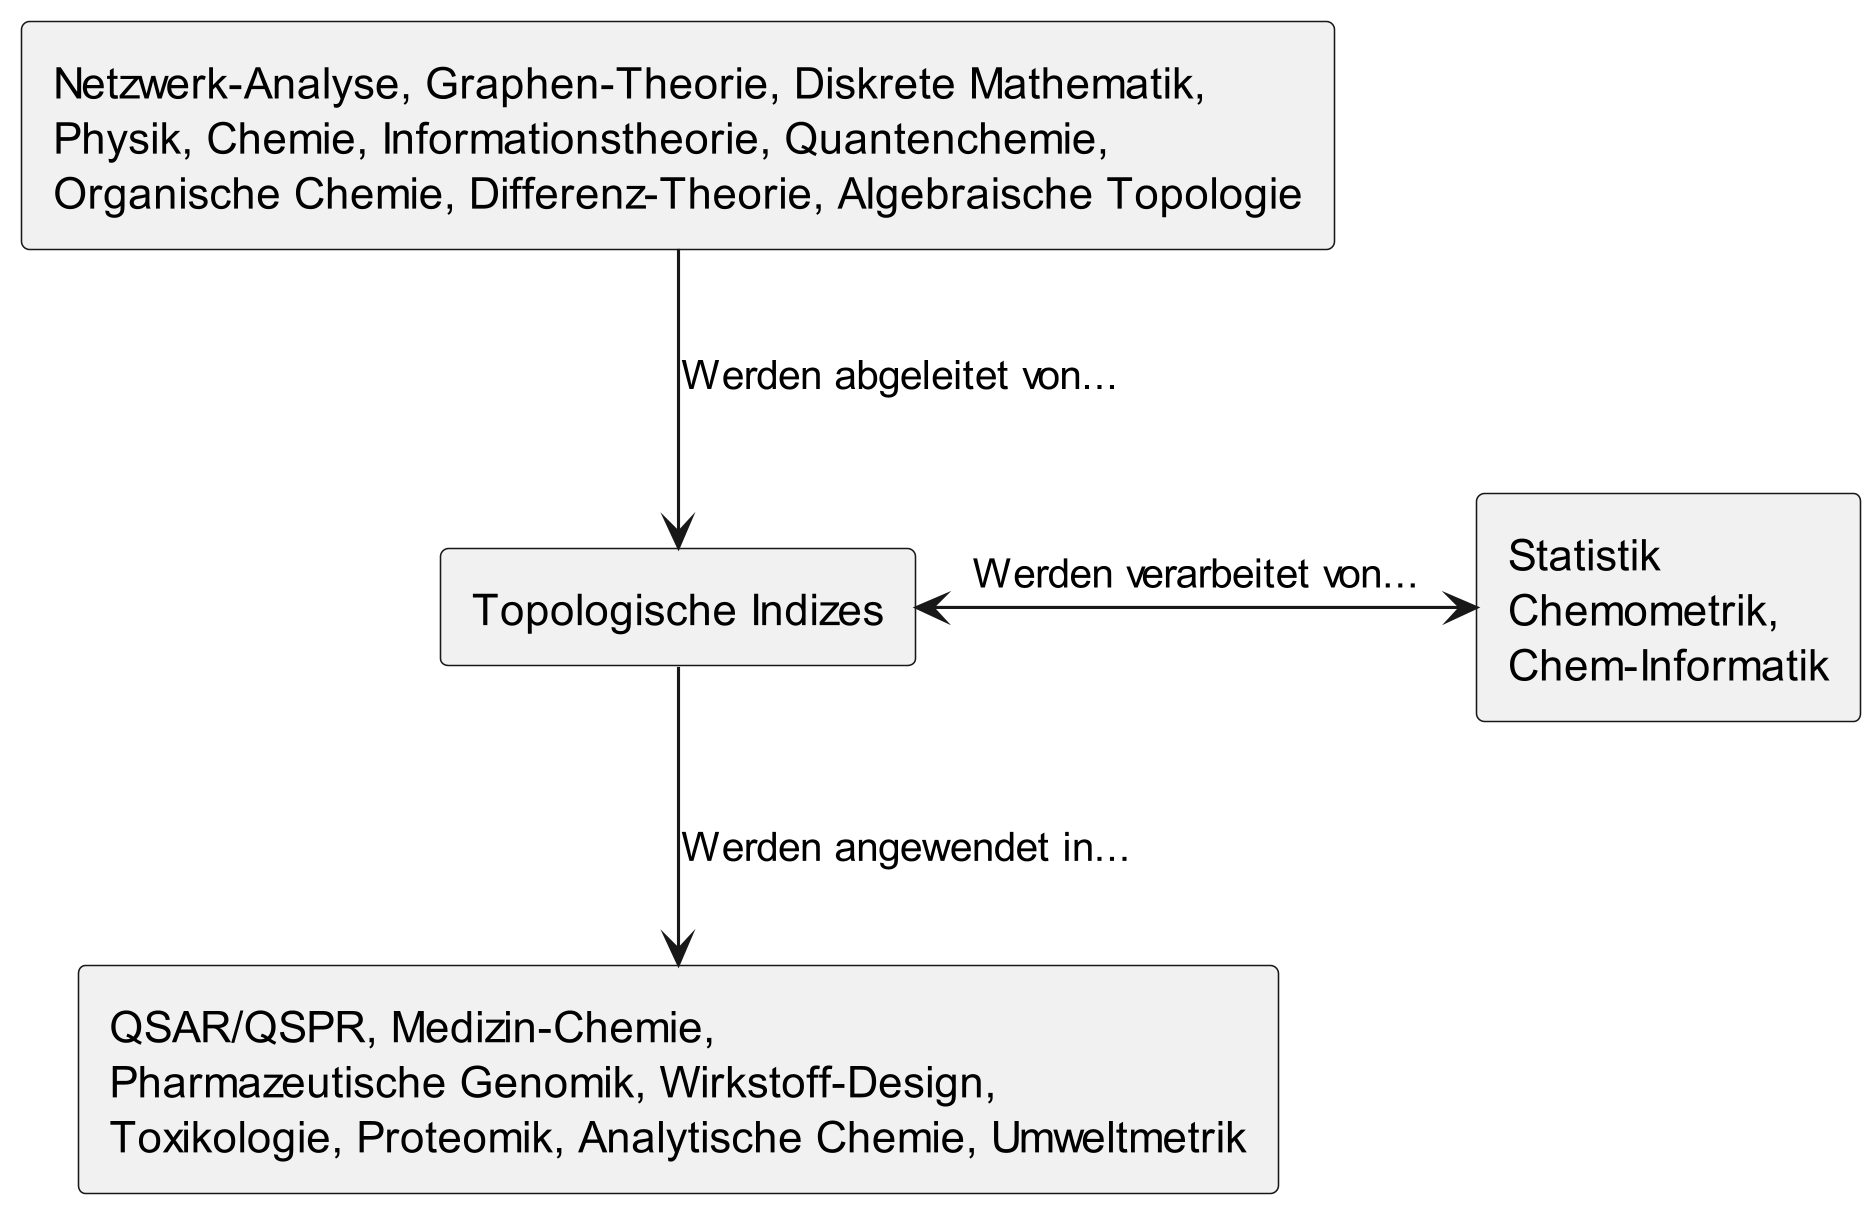
\includegraphics[width=0.9\textwidth]{images/10_introduction/overview_molecule_descriptor.png}
    \caption{Übersicht zur Anordnung des Themengebietes, übersetzt aus Todeschini und Consonni \cite{todeschini_handbook_2000}}
    \label{fig:overview_indices}
\end{figure}

Eine der Hauptanwendungen der Graphentheorie ist die Darstellung und Analyse von Netzwerken.
Beispielsweise kann ein soziales Netzwerk als Graph dargestellt werden, mit Menschen als Knoten und den Beziehungen zwischen ihnen (Freundschaften, familiäre Bindungen etc.) als Kanten.
Die Analyse der Struktur des Netzwerks kann Aufschluss darüber geben, wie sich Informationen im Netzwerk verbreiten und welche Faktoren die Veränderung des Netzwerks beeinflussen können \cite[p.~440ff.]{watts_collective_1998}.

Die Graphentheorie wird auch dazu verwendet, Probleme in der Informatik und den Ingenieurwissenschaften zu lösen.
Sie kann etwa genutzt werden, um den kürzesten Weg zwischen zwei Punkten in einem Verkehrsnetz zu finden \cite[p.~269]{dijkstra_note_1959} oder um Aufgaben in einem Computersystem zu planen \cite[p.~9]{garey_computers_1990}.
In der Biologie kann die Graphentheorie eingesetzt werden, um die Wechselwirkungen zwischen Genen oder Proteinen in einer Zelle zu untersuchen \cite[p.~3]{albert_diameter_1999} und in der Soziologie, um die Struktur sozialer Netzwerke und deren Kommunikationsmuster zu analysieren \cite[p.~1ff.]{barnes_graph_1969}.

\section{Was ist ein Graph?}

Formell wird ein Graph als $G = (V, E)$ definiert, wobei $V$ die Menge der Knoten und $E$ die Menge der Kanten ist.
Knoten können als Punkte oder Kreise dargestellt werden und Kanten als Linien, die zwei Knoten verbinden \cite[p.~45]{barabasi_network_2016}.

Ein Graph kann \textbf{\textit{ungerichtet}} oder \textbf{\textit{gerichtet}} sein. Bei einem ungerichteten Graphen können die Kanten in beide Richtungen durchlaufen werden.
Bei einem gerichteten Graphen können die Kanten nur in eine Richtung durchlaufen werden.
Eine Kante kann auch \textbf{\textit{gewichtet}} oder \textbf{\textit{ungewichtet}} sein.
Gewichtete Kanten haben einen numerischen Wert, der als Kosten, Länge oder ähnliches interpretiert werden kann \cite[p.~46]{barabasi_network_2016}.

Auf Abbildung \ref{fig:general_graphs} folgt ein Beispiel für einen gerichteten, ungerichtet und gewichteten Graphen.

\begin{figure}[H]
    \centering
    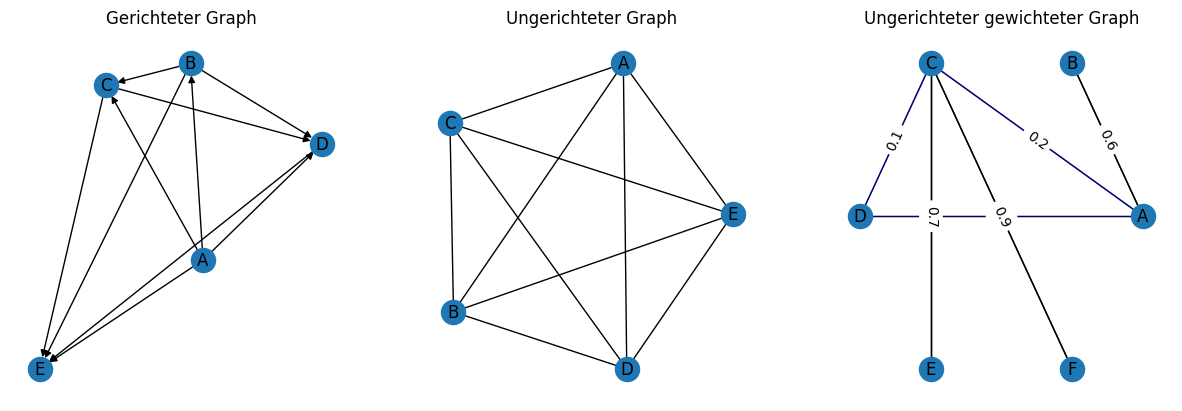
\includegraphics[width=0.9\textwidth]{images/10_introduction/graph_intro.png}
    \caption{Darstellung der verschiedenen Graphen}
    \label{fig:general_graphs}
\end{figure}

Ein Graph kann \textbf{\textit{zusammenhängend}} oder \textbf{\textit{unzusammenhängend}} sein.
Ein zusammenhängender Graph besteht aus einer einzigen zusammenhängenden Komponente, d. h. es gibt einen Pfad von jedem Knoten zu jedem anderen Knoten.
Ein unzusammenhängender Graph besteht aus mehreren Komponenten, die nicht miteinander verbunden sind.

Die \textbf{\textit{Ordnung}} eines Graphen ist die Anzahl der Knoten, die in ihm enthalten sind.
Die Grösse eines Graphen ist die Anzahl der Kanten, die in ihm enthalten sind.
Ein Graph mit $n$ Knoten kann höchstens $\frac{n(n-1)}{2}$ Kanten enthalten, wenn es sich um einen ungerichteten Graphen handelt \cite[p.~48]{barabasi_network_2016}.
Wenn es sich um einen gerichteten Graphen handelt, kann es höchstens $n(n-1)$ Kanten enthalten.

Ein wichtiger Begriff in der Graphentheorie ist der \textbf{\textit{Grad}} eines Knotens, der die Anzahl der Kanten beschreibt, die mit diesem Knoten verbunden sind. Im Falle eines ungerichteten Graphen ist der Grad eines Knotens einfach die Anzahl seiner Nachbarn. Im Falle eines gerichteten Graphen unterscheidet man zwischen dem Eingangsgrad, der Anzahl der Kanten, die auf den Knoten zeigen, und dem Ausgangsgrad, der Anzahl der Kanten, die vom Knoten wegführen. Der Grad eines Knotens kann dazu verwendet werden, die Verbindungsstärke zwischen den Knoten zu beschreiben und somit eine Aussage über die Struktur des Graphen zu treffen \cite[p.~48]{barabasi_network_2016} \cite[p.~14]{harary_graph_1994}.

Eine Möglichkeit, die Verbindungen zwischen den Knoten eines Graphen darzustellen, ist die Verwendung von \textbf{\textit{Adjazenzmatrizen}}. Eine Adjazenzmatrix ist eine quadratische Matrix, die die Verbindungen zwischen den Knoten des Graphen darstellt. Die Einträge der Matrix geben an, ob es eine Verbindung zwischen zwei Knoten gibt oder nicht. Im Falle eines ungerichteten Graphen ist die Adjazenzmatrix symmetrisch. Im Falle eines gerichteten Graphen ist die Adjazenzmatrix nicht symmetrisch. Die Verwendung von Adjazenzmatrizen kann helfen, die Struktur des Graphen zu verstehen und somit Aussagen über seine Eigenschaften und Funktionen zu treffen \cite[p.~51]{barabasi_network_2016} \cite[p.~151]{harary_graph_1994}.

Als Beispiel betrachten wir einen ungerichteten Graphen mit 4 Knoten, der wie folgt dargestellt werden kann:

\[
    A =
    \begin{bmatrix}
        0 & 1 & 1 & 0 \\
        1 & 0 & 1 & 0 \\
        1 & 1 & 0 & 1 \\
        0 & 0 & 1 & 0
    \end{bmatrix}
\]

In diesem Fall ist die Adjazenzmatrix symmetrisch, da der Graph ungerichtet ist. Die Einträge der Matrix geben an, ob es eine Verbindung zwischen zwei Knoten gibt oder nicht. Es gibt so etwa eine Verbindung zwischen Knoten 1 und Knoten 2, da der Eintrag $a_{1,2} = 1$ ist. Es gibt jedoch keine Verbindung zwischen Knoten 1 und Knoten 4, da der Eintrag $a_{1,4} = 0$ ist. Die Verwendung der Adjazenzmatrix kann helfen, die Struktur des Graphen zu visualisieren und Aussagen über seine Eigenschaften zu treffen.

Ein weiterer wichtiger Begriff in der Graphentheorie ist der \textbf{\textit{durchschnittliche Grad}} des Graphen, der angibt, wie viele Kanten jeder Knoten im Durchschnitt hat \cite[p.~48]{barabasi_network_2016}. Für einen ungerichteten Graphen mit $n$ Knoten und $m$ Kanten wird der durchschnittliche Grad $k$ wie folgt definiert:

$$k = \frac{2m}{n}$$

Für gerichtete Graphen unterscheidet man zwischen dem durchschnittlichen Eingangsgrad und dem durchschnittlichen Ausgangsgrad. Der durchschnittliche Grad gibt eine Aussage über die allgemeine Verbindungsstärke im Graphen und kann bei der Identifikation von Clusterstrukturen oder dem Vergleich von Graphen helfen \cite[p.~48]{barabasi_network_2016}.

Ein weiteres wichtiges Konzept in der Graphentheorie ist die \textbf{\textit{Gradverteilung}}. Die Gradverteilung beschreibt, wie viele Knoten in einem Graphen einen bestimmten Grad haben.

$$ P(k) := \frac{\delta_k}{N}$$

Wobei $|V| := N$ und $ \delta_k $ die Anzahl der Knoten mit Grad $k$ ist \cite[p.~311]{emmert-streib_mathematical_2020}.

Eine häufige Gradverteilung ist die Poisson-Verteilung, die für viele zufällige Graphen gilt. Eine andere häufige Gradverteilung ist die Potenzgesetz-Verteilung, die für viele reale Netzwerke gilt, wie in sozialen Netzwerken oder in der Biologie. Die Potenzgesetz-Verteilung ist charakterisiert durch einen hohen Anteil von Knoten mit niedrigem Grad und einem kleinen Anteil von Knoten mit hohem Grad, die als Hubs bezeichnet werden. Die Gradverteilung kann helfen, die Struktur eines Graphen zu verstehen und somit Aussagen über die Funktionsweise des Graphen zu treffen \cite[p.~51]{barabasi_network_2016}.

Die Zentralitätsmasse beschreiben, welche Knoten im Graphen besonders wichtig sind \cite[p.~313]{emmert-streib_mathematical_2020}.
Die Zentralität eines Knotens kann auf verschiedene Arten gemessen werden.
Eine Möglichkeit ist die \textbf{\textit{Degree-Zentralität}}, die angibt, wie viele Kanten mit einem Knoten verbunden sind.
Ein Knoten mit hoher Degree-Zentralität hat viele Nachbarn und ist somit wichtiger als ein Knoten mit niedriger Degree-Zentralität.
Die Degree-Zentralität $C_D(v)$ eines Knotens $v$ in einem ungerichteten Graphen $G=(V,E)$ wird wie folgt definiert:

$$C_D(v) = k_v$$

wobei $k_v$ die Anzahl der Nachbarn von $v$ ist \cite[p.~314]{emmert-streib_mathematical_2020}.

Ein weiteres Mass für die Zentralität ist die \textbf{\textit{Betweenness-Zentralität}}, die angibt, wie oft ein Knoten auf dem kürzesten Pfad zwischen anderen Knoten liegt.
Ein Knoten mit hoher Betweenness-Zentralität spielt eine wichtige Rolle bei der Vermittlung von Information zwischen anderen Knoten.
Die Betweenness-Zentralität $C_B(v)$ eines Knotens $v$ in einem ungerichteten Graphen $G=(V,E)$ wird wie folgt definiert:

$$C_B(v_k) = \sum_{v_i, v_j \in V, v_i \ne v_j} \frac{\sigma_{v_i v_j}(v_k)}{\sigma_{v_i v_j}}$$

wobei $\sigma_{v_i v_j}$ die Anzahl der kürzesten Pfade von $v_i$ nach $v_j$ ist und $\sigma_{v_i v_j}(v_k)$ die Anzahl der kürzesten Pfade von $v_i$ nach $v_j$ durch $v_k$ ist \cite[p.~314]{emmert-streib_mathematical_2020}.
